% Página 63 do PDF de Gabriel
\begin{frame}[plain,noframenumbering,label=original-63]
  \begin{tikzpicture}[remember picture,overlay,x=1bp,y=-1bp]
  \begin{scope}[shift={(current page.north west)}]
  \Fundo{63}
  \Texto{44.456}{41.894}{111.824}{8.518}{b}{34E0C8}{SÍNTESE E CONTINUIDADE}
  \Texto{43.039}{116.125}{63.147}{56.787}{b}{FFB014}{08}
  \Texto{43.039}{155.148}{215.44}{24.608}{b}{FFFFFF}{Síntese da análise}
  \Texto{43.039}{234.662}{46.285}{7.572}{b}{34E0C8}{EMASC 2026}
  \Texto{91.429}{234.662}{2.65}{7.572}{b}{FFB014}{\textbullet{}}
  \Texto{96.176}{234.662}{21.45}{7.572}{b}{34E0C8}{LAME}
  \Link{42.042}{135.586}{217.431}{20.866}{original-63}
  \end{scope}
  \end{tikzpicture}
\end{frame}


% Página 64 do PDF de Gabriel
\begin{frame}[plain,noframenumbering,label=original-64]
  
\begin{tikzpicture}[remember picture,overlay,x=1bp,y=-1bp]
  \begin{scope}[shift={(current page.north west)}]
  \Fundo{64}
  \Texto{40.175}{27.942}{190.525}{17.983}{b}{2C2084}{Principais conclusões}
  \Texto{35.433}{63.506}{175.76}{8.518}{i}{737696}{Quatro práticas resumem o percurso do curso.}
  \Texto{28.574}{100.642}{42.145}{9.465}{b}{027499}{1. Validar}
  \Texto{28.574}{115.586}{67.87}{9.465}{r}{000000}{A qualidade dos}
  \Texto{28.574}{127.542}{67.349}{9.465}{r}{000000}{dados antecede}
  \Texto{28.574}{139.497}{39.599}{9.465}{r}{000000}{o cálculo.}
  \Texto{137.268}{100.642}{56.768}{9.465}{b}{007078}{2. Dispersão}
  \Texto{137.268}{115.586}{67.331}{9.465}{r}{000000}{A média isolada}
  \Texto{137.268}{127.542}{57.866}{9.465}{r}{000000}{é insuficiente:}
  \Texto{137.268}{139.497}{44.19}{9.465}{r}{000000}{mediana e}
  \Texto{137.268}{151.452}{41.029}{9.465}{r}{000000}{dispersão}
  \Texto{137.268}{163.407}{54.175}{9.465}{r}{000000}{completam o}
  \Texto{137.268}{175.362}{33.807}{9.465}{r}{000000}{resumo.}
  \Texto{245.963}{100.879}{44.284}{9.465}{b}{231A6A}{3. Gráfico}
  \Texto{245.963}{115.823}{38.303}{9.465}{r}{000000}{O gráfico}
  \Texto{245.963}{127.778}{46.83}{9.465}{r}{000000}{antecede o}
  \Texto{245.963}{139.733}{47.729}{9.465}{r}{000000}{coeficiente.}
  \Texto{354.657}{100.642}{39.552}{9.465}{b}{CC8D10}{4. Causa}
  \Texto{354.657}{115.586}{66.81}{9.465}{r}{000000}{Associação não}
  \Texto{354.657}{127.541}{29.444}{9.465}{r}{000000}{implica}
  \Texto{354.657}{139.497}{52.992}{9.465}{r}{000000}{causalidade.}
  \Texto{37.21}{247.463}{40.499}{6.625}{b}{737696}{EMASC 2026}
  \Texto{80.653}{247.463}{2.319}{6.625}{r}{FFB014}{\textbullet{}}
  \Texto{85.914}{247.463}{117.821}{6.625}{r}{737696}{Liga Acadêmica Matemática \& Empresa}
  \Texto{206.683}{247.463}{2.319}{6.625}{r}{FFB014}{\textbullet{}}
  \Texto{211.943}{247.463}{13.25}{6.625}{r}{737696}{UFS}
  \Texto{397.549}{248.132}{7.367}{6.625}{b}{2C2084}{39}
  \Texto{406.02}{248.132}{10.315}{6.625}{r}{737696}{/ 40}
  \end{scope}
  \end{tikzpicture}
\end{frame}


% Página 65 do PDF de Gabriel
\begin{frame}[plain,noframenumbering,label=original-65]
  
\begin{tikzpicture}[remember picture,overlay,x=1bp,y=-1bp]
  \begin{scope}[shift={(current page.north west)}]
  \Fundo{65}
  \Texto{40.175}{28.167}{149.902}{17.983}{b}{2C2084}{Próximos passos}
  \Texto{35.433}{63.506}{215.361}{8.518}{i}{737696}{Descrever os dados abre caminho para estimar e decidir.}
  \Texto{38.534}{100.879}{75.555}{9.465}{b}{231A6A}{Análise preditiva}
  \Texto{38.534}{115.823}{137.481}{9.465}{r}{000000}{Estimar valores não observados.}
  \Texto{38.534}{131.763}{162.975}{8.518}{r}{737696}{Ex.: prever a pontuação de saúde mental a}
  \Texto{38.534}{143.718}{122.881}{8.518}{r}{737696}{partir das horas de uso de redes}
  \Texto{38.534}{155.674}{45.827}{8.518}{r}{737696}{(regressão).}
  \Texto{250.943}{100.879}{83.979}{9.465}{b}{CC8D10}{Análise prescritiva}
  \Texto{250.943}{115.823}{132.408}{9.465}{r}{000000}{Recomendar ações a partir das}
  \Texto{250.943}{127.778}{49.584}{9.465}{r}{000000}{estimativas.}
  \Texto{250.943}{143.718}{147.319}{8.518}{r}{737696}{Ex.: definir limites de uso associados a}
  \Texto{250.943}{155.674}{113.119}{8.518}{r}{737696}{maior bem-estar (otimização).}
  \Texto{49.227}{187.282}{294.28}{8.518}{r}{000000}{Ambas exigem dados confiáveis e, no caso de recomendações, evidência de}
  \Texto{346.268}{187.282}{48.766}{8.518}{b}{000000}{causalidade}
  \Texto{397.791}{187.282}{8.518}{8.518}{r}{000000}{\textemdash{}}
  \Texto{49.227}{198.241}{91.517}{8.518}{r}{000000}{não apenas associação.}
  \Texto{35.433}{217.652}{168.079}{6.625}{r}{737696}{Para continuar: documentação do pandas e do seaborn \textbullet{}}
  \Texto{205.352}{217.652}{109.082}{6.625}{i}{737696}{Practical Statistics for Data Scientists}
  \Texto{316.467}{217.652}{47.323}{6.625}{r}{737696}{(Bruce \& Bruce)}
  \Texto{37.21}{247.463}{40.499}{6.625}{b}{737696}{EMASC 2026}
  \Texto{80.653}{247.463}{2.319}{6.625}{r}{FFB014}{\textbullet{}}
  \Texto{85.913}{247.463}{117.821}{6.625}{r}{737696}{Liga Acadêmica Matemática \& Empresa}
  \Texto{206.682}{247.463}{2.319}{6.625}{r}{FFB014}{\textbullet{}}
  \Texto{211.943}{247.463}{13.25}{6.625}{r}{737696}{UFS}
  \Texto{397.549}{248.132}{7.367}{6.625}{b}{2C2084}{40}
  \Texto{406.02}{248.132}{10.315}{6.625}{r}{737696}{/ 40}
  \end{scope}
  \end{tikzpicture}
\end{frame}
